\documentclass[border=0cm]{standalone}
\usepackage{xcolor}
\usepackage{tikz}
\usetikzlibrary{arrows, arrows.meta}
\tikzset{    
    barbarrow/.style={ % style that just defines the arrow tip
        %>={Straight Barb[left,length=5pt,width=5pt]},
        >={Triangle[left,length=5pt,width=5pt]},
        double,
        semithick,
        <->
    },
    whites/.style={
        thick, 
        color=white
    }
}
\definecolor{light-gray}{gray}{0.975}
\definecolor{pcolor}{rgb}{0.21, 0.27, 0.31}
\definecolor{purple}{rgb}{1.0, 0.0 1.0}
\definecolor{pgreen}{rgb}{0.0, 0.5 0.0}
\begin{document}
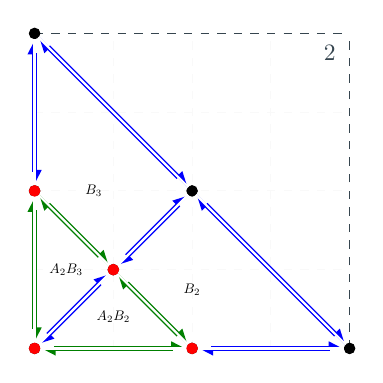
\begin{tikzpicture}
    \tikzstyle{node1}=[draw,scale=0.4,shape=circle,color=black,fill=black]
    \tikzstyle{node2}=[draw,scale=0.4,shape=circle,color=red,fill=red]
    \tikzstyle{nodePurple}=[draw,scale=0.4,shape=circle,color=red,fill=red]
    \tikzstyle{text}=[draw,scale=0.5,color=black]
    \draw[color=light-gray, style=dashed] (4,4) grid (8,8);
    \draw[color=pcolor, style=dashed, step=4] (4,4) grid (8,8);
    \node[scale=0.85, color = pcolor] at (7.75, 7.75) {$2$};
    
    \node[node1] (M) at (4,6) {};
    \node[node1] (R) at (6,4) {};
    \node[node1] (Z) at (4,4) {};
    \node[node1] (N) at (4,8) {};
    \node[node1] (S) at (6,6) {};
    \node[node1] (T) at (8,4) {};
    \node[node1] (U) at (5,5) {};

    \draw[barbarrow, color=blue] (Z) -- (U); 
    \draw[barbarrow, color=blue] (U) -- (S); 
    \draw[barbarrow, color=blue] (N) -- (S); 
    \draw[barbarrow, color=blue] (S) -- (T);
    \draw[barbarrow, color=blue] (R) -- (T);
    \draw[barbarrow, color=blue] (M) -- (N);

    \draw[whites] (Z) -- (U); 
    \draw[whites] (U) -- (S); 
    \draw[whites] (N) -- (S); 
    \draw[whites] (S) -- (T);
    \draw[whites] (R) -- (T);
    \draw[whites] (M) -- (N);
    
    \draw[barbarrow, color=pgreen] (M) -- (U);
    \draw[barbarrow, color=pgreen] (U) -- (R);
    \draw[whites] (M) -- (U);
    \draw[whites] (U) -- (R);

    \draw[barbarrow, color=pgreen](Z) -- (M);
    \draw[barbarrow, color=pgreen] (Z) -- (R);
    \draw[whites](Z) -- (M);
    \draw[whites] (Z) -- (R);

    \node[nodePurple] (M2) at (4,6) {};
    \node[nodePurple] (R2) at (6,4) {};
    \node[nodePurple] (U2) at (5,5) {};
    \node[nodePurple] (Z2) at (4,4) {};

    \node[scale=0.5] at (4.4,5) {$A_2B_3$};
    \node[scale=0.5] at (5,4.4) {$A_2B_2$};
    \node[scale=0.5] at (6,4.75) {$B_2$};
    \node[scale=0.5] at (4.75,6) {$B_3$};
    
\end{tikzpicture}
\end{document}
